\section{Concurrent execution}


\subsection{Parallelism vs Concurrency}


\begin{figure}
    \centering
    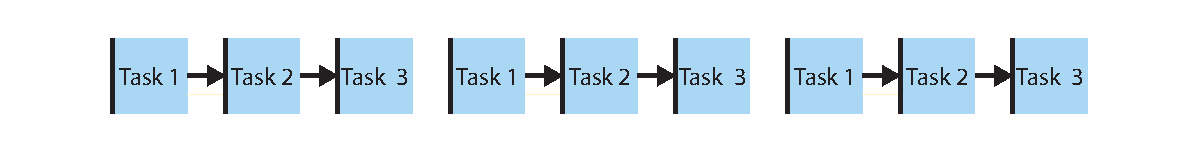
\includegraphics[width=\textwidth]{figures/concurrency/sequential.pdf}
    \caption{Visualisation of a sequential execution.}
    \label{fig:concurrency_sequential}
\end{figure}

\begin{figure}
    \centering
    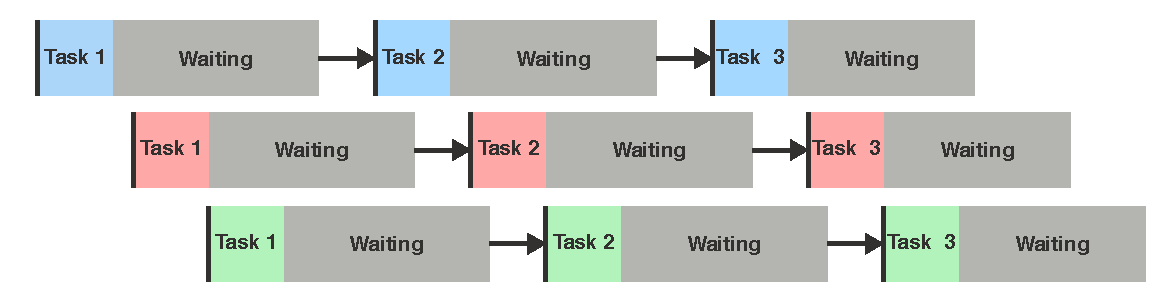
\includegraphics[width=\textwidth]{figures/concurrency/concurrent.pdf}
    \caption{Visualisation of a concurrent execution.}
    \label{fig:concurrency_concurrent}
\end{figure}

\begin{figure}
    \centering
    
\includegraphics[width=\textwidth]{figures/concurrency/paralell.pdf}
    \caption{Visualisation of a parallel execution.}
    \label{fig:concurrency_parallel}
\end{figure}

\subsection{Context switching}

\subsection{Parallel execution}

\subsection{In python}
% \begin{listing}[H]
%     \begin{minted}{python}
%         import asyncio, threading, time
%         from concurrent.futures import ThreadPoolExecutor

%         def do_nothing(): time.sleep(1)
%         async def do_nothing_async(): await asyncio.sleep(1)

%         async def test_asyncio():
%             await asyncio.gather(*[do_nothing_async() for _ in range(N)])

%         def test_thread_pool():
%             with ThreadPoolExecutor(max_workers=10000) as ex:
%                 futures = [ex.submit(do_nothing) for _ in range(N)]

%         async def test_thread_pool_async():
%             loop = asyncio.get_event_loop()
%             with ThreadPoolExecutor(max_workers=10000) as ex:
%                 asyncio.gather(*[loop.run_in_executor(ex, do_nothing) for _ in range(10000)])

%         def test_threads():
%             threads = [threading.Thread(target=do_nothing) for _ in range(10000)]
%             [thread.start() for thread in threads]
%             [thread.join() for thread in threads]

%         def perf_test(func: callable):
%             start_time = time.perf_counter()
%             asyncio.run(func()) if asyncio.iscoroutinefunction(func) else func()
%             end_time = time.perf_counter()
%             print(f"{func.__name__} took {end_time - start_time:.6f} seconds to complete.")

%         if __name__ == "__main__":
%             perf_test(test_asyncio)
%             perf_test(test_thread_pool)
%             perf_test(test_thread_pool_async)
%             perf_test(test_threads)
%     \end{minted}
%     \caption{Code used to compatre asyncio and threads.}
%     \label{listing:concurrency_test}
% \end{listing}
\begin{listing}
    \begin{minted}{bash}
        >>> test_asyncio took 1.373797 seconds to complete.
        >>> test_thread_pool took 4.091199 seconds to complete.
        >>> test_thread_pool_async took 4.391777 seconds to complete.
        >>> test_threads took 5.373108 seconds to complete.
    \end{minted}
    \caption{Results when running the code in Listing  \ref{listing:concurrency_test} on the \jx}
\end{listing}
% \begin{listing}[H]
%     \begin{minted}{python}
%         import asyncio, threading, time

%         def do_nothing(): pass
%         async def do_nothing_async(): pass

%         async def test_asyncio():
%             start_time = time.perf_counter()
%             await asyncio.gather(*[do_nothing_async() for _ in range(10000)])
%             end_time = time.perf_counter()
%             print(f"Asyncio took {end_time - start_time:.6f} seconds to complete.")

%         def test_threads():
%             threads = [threading.Thread(target=do_nothing) for _ in range(10000)]
%             start_time = time.perf_counter()
%             for thread in threads:
%                 thread.start()
%             for thread in threads:
%                 thread.join()
%             end_time = time.perf_counter()
%             print(f"Threads took {end_time - start_time:.6f} seconds to complete.")

%         if __name__ == "__main__":
%             asyncio.run(test_asyncio())
%             test_threads()
%     \end{minted}
%     \begin{minted}{bash}
%         >>> Asyncio took 0.311703 seconds to complete.
%         >>> Threads took 11.898036 seconds to complete.
%     \end{minted}
%     \caption{Comparison of asyncio and threads running on INTEL i7-11800H @ 2.30GHz.}
% \end{listing}

\subsection{Message passing}
\subsubsection{}
\begin{itemize}
    \item Can the task be done in parallel?
    \item Does the task require a lot of memory?
    \item Does the order of output matter?
    \item Is latency an issue?
    \item Is there any bottlenecks?
    \item What tasks are resource intensive?

\end{itemize}